\documentclass[10pt,a4paper,onecolumn]{article}
\usepackage[utf8]{inputenc}
\usepackage[T1]{fontenc}
\usepackage{newtxtext,newtxmath}
\usepackage[top=2.4cm,bottom=2.4cm,left=3.2cm,right=2.0cm]{geometry}
\usepackage{mathtools}
\usepackage{amsmath}
\DeclareMathOperator*{\argmax}{arg\,max}
\DeclareMathOperator*{\argmin}{arg\,min}
\DeclareMathOperator{\diag}{diag}
\usepackage{amsthm}
\theoremstyle{definition}
\newtheorem{definition}{Definition}
\usepackage{booktabs}
\usepackage{array}
\usepackage{multirow}
\usepackage{tabularx}
\usepackage{longtable}
\usepackage{enumitem}
\usepackage{titlesec}
\usepackage{caption}
\captionsetup{font=small,labelfont=bf,labelsep=period,justification=raggedright,singlelinecheck=false}
\titlespacing*{\section}{0pt}{2.2ex plus 0.6ex minus 0.3ex}{1.0ex}
\titlespacing*{\subsection}{0pt}{1.8ex plus 0.4ex minus 0.2ex}{0.8ex}
\titlespacing*{\subsubsection}{0pt}{1.4ex plus 0.3ex minus 0.2ex}{0.6ex}
\titleformat{\section}{\large\bfseries}{\thesection.}{0.5em}{}
\titleformat{\subsection}{\normalsize\bfseries\itshape}{\thesubsection.}{0.5em}{}
\titleformat{\subsubsection}{\normalsize\itshape}{\thesubsubsection.}{0.5em}{}

\usepackage{tikz}
\usepackage{pgfplots}
\pgfplotsset{compat=1.18}
\usetikzlibrary{
  arrows.meta,
  positioning,
  shapes.geometric,
  shadows,
  fit,
  calc,
  matrix,
  shapes.misc,
  shapes.symbols
}
\usepackage{algorithm}
\usepackage{algorithmicx}
\usepackage{algpseudocode}
\algrenewcommand\algorithmicrequire{\textbf{Input:}}
\algrenewcommand\algorithmicensure{\textbf{Output:}}
\usepackage{graphicx}
\usepackage{adjustbox}
\usepackage{url}
\usepackage{xcolor}
\usepackage{cite}
\usepackage[colorlinks=true,allcolors=blue!60!black]{hyperref}
\usepackage{placeins}
\usepackage{fancyhdr}

\pagestyle{fancy}
\fancyhf{}
\fancyhead[L]{\footnotesize\textit{Electronics} \textbf{2026}, \textit{15}, x}
\fancyhead[R]{\footnotesize\thepage}
\renewcommand{\headrulewidth}{0.4pt}
\setlength{\parindent}{1.2em}
\setlength{\parskip}{0.35em}
\renewcommand{\baselinestretch}{1.08}

\hypersetup{pdftitle={Verified Localized Episodic Grounding for Auditable LLM-Assisted Network Traffic Analysis: Counterexample Diagnosis and Gating}}

\begin{document}

\noindent{\footnotesize\textit{Article}}\\[0.4em]
{\LARGE\bfseries Verified Localized Episodic Grounding for Auditable LLM-Assisted Network Traffic Analysis: Counterexample Diagnosis and Gating\par}
\vspace{0.8em}

\noindent{\bfseries Ye Tang$^{1,\dagger}$, Ruikai Han$^{1,\dagger}$, Yi Hu$^{1}$ and Ruzhen Chen$^{2,}$*}\\[0.4em]
{\small
$^{1}$ School of Information Science and Technology, Xizang University, Lhasa 850000, China; 3441691137@qq.com (Y.T.); 1763683932@qq.com (R.H.); hy610400@163.com (Y.H.)\\
$^{2}$ School of Education, Xizang University, Lhasa 850000, China\\
$^{*}$ Correspondence: crz@xzu.edu.cn\\
$^{\dagger}$ These authors contributed equally to this work.
}

\vspace{0.8em}
\hrule
\vspace{0.6em}
\noindent\textbf{Abstract:} Memory-augmented large language models (LLMs) can assist network intrusion triage by retrieving historical flows without parameter updates, yet compressing raw telemetry into natural-language rules creates a fundamental tension between single-record faithfulness and cross-flow specificity. We present Verified Localized Episodic Grounding (VLEG), an auditable memory-consolidation and hybrid-inference framework that verifies candidate reflections against their labeled source records within a bounded refinement budget $K$ and pairs admitted rules with raw flow evidence. In a 16-scene symbolic sanity check at 7B and 70B scales, bounded verification eliminates source-label inversions ($100\%$ observed source-label agreement on admitted episodes versus $41.7\%$--$50.0\%$ for unverified proposals), reaching accuracy comparable to raw in-context retrieval at 70B ($91.67\%$ versus $89.58\%$, $44/48$ versus $43/48$) while trailing raw retrieval at 7B ($75.0\%$ versus $87.5\%$). On a 32-episode few-shot benchmark over 1000 deduplicated UNSW-NB15 test fingerprints across five memory seeds, unverified single-step reflection mislabels $95.0\%$ ($76/80$) of malicious historical flows as benign, causing attack recall to collapse to $6.17\%$ ($42.66\%$ Macro-F1). Standard VLEG ($K=3$) restores $100\%$ source-label agreement ($158/158$) and raises attack recall to $77.74\%$ and Macro-F1 to $59.68\%$ ($+17.02$ percentage points, pp), but trails zero-cost raw flow retrieval ($63.92\%$ Macro-F1) by $4.24$~pp due to a $48.78\%$ false positive rate (FPR). Using a deterministic counterexample compiler that parses $99.4\%$ ($157/158$) of admitted rules into executable Boolean predicates, we show that $72.0\%$ ($113/157$) of source-consistent rules match contrary-label historical flows. Integrating this compiler as a within-seed counterexample gate (VLEG-CG) without additional LLM calls reduces the FPR by $9.35$--$10.92$~pp (down to $37.86\%$--$39.43\%$, comparable to 32-flow Random Forest at $40.66\%$ and GBDT at $39.22\%$) and recovers Macro-F1 to $63.32\%$--$63.55\%$.

\vspace{0.4em}
\noindent\textbf{Keywords:} episodic memory; hallucination mitigation; large language models; network traffic analysis; intrusion detection; rule over-generalization; verified memory consolidation
\vspace{0.6em}
\hrule
\vspace{1.0em}

\section{Introduction}
\subsection{Background and Motivation}
Large language models (LLMs) can use in-context demonstrations to support classification and incident analysis without parameter updates \cite{brown2020language,lewis2020retrieval}. In network traffic analysis and Security Operations Center (SOC) intrusion triage \cite{lin2022etbert,sharafaldin2018cicids,houssel2024explainable,islam2026maids}, security teams increasingly explore LLM agents to link novel flow telemetry to historical incidents via human-auditable verbal rules. Whereas traditional supervised classifiers such as Random Forest (RF) and Gradient Boosting Decision Trees (GBDT) excel at high-throughput binary filtering when trained on tens of thousands of labeled flows, cold-start triage often operates with only a small curated bank of investigated episodes where analysts require explicit rule rationales. However, finite and imperfectly utilized context windows make the selection and verification of this historical evidence critical \cite{an2024why,liu2024lost}.

Persistent-memory architectures extend an agent's access to experience beyond the current prompt \cite{packer2023memgpt,wang2023longmem,wang2024memoryllm,gutierrez2024hipporag,maharana2024evaluating}. Retaining raw flow records preserves instance-level detail, whereas converting records into natural-language reflections or global summaries supplies compact decision heuristics. Yet rule compression introduces two distinct failure modes: (1) unverified reflections generated without label supervision can hallucinate class labels, and (2) locally verified reflections that accurately describe a single source flow can still assert overly broad conditions that trigger false alarms across benign background traffic.

Crucially, single-episode source fidelity and cross-episode specificity are distinct requirements. Checking a candidate explanation against its originating record alone can catch label inversions or fabricated attributes, but cannot determine whether the selected feature thresholds separate classes across the broader traffic distribution. Evaluating reflective memory systems therefore requires auditing admission coverage, source-label agreement, cross-episode counterexample rates, and downstream classification trade-offs together.

\subsection{Research Positioning and Study Scope}
Memory-augmented language models retain and reuse experience through episodic retrieval, local reflection, and global semantic consolidation \cite{wu2025from,zhang2024survey}. Feedback-driven agents revise behavior using trial rewards \cite{shinn2023reflexion,wang2024voyager}, while global hypothesis frameworks synthesize and verify rules across multiple records \cite{agarwal2026hypothesis,he2024idea}. Rather than claiming that LLM reflection outperforms supervised tabular classifiers or raw retrieval in unconditional accuracy, this study conducts a rigorous diagnostic audit of per-episode verification, rule over-generalization, and counterexample gating under strict few-shot memory budgets.

Specifically, we address three engineering questions:
\begin{enumerate}[leftmargin=1.8em]
    \item Does checking each local reflection against its labeled source episode before memory admission prevent the label-inversion and recall collapse of unverified reflection?
    \item Why do $100\%$ source-consistent local rules still elevate false alarms when paired with raw telemetry on deduplicated network flows?
    \item Can a deterministic counterexample compiler screen out over-generalized local rules within the historical memory bank to suppress false positives without extra LLM calls?
\end{enumerate}

\subsection{Proposed VLEG Framework and Counterexample Gate}
We propose Verified Localized Episodic Grounding (VLEG), an inspectable memory-consolidation and hybrid-inference framework paired with a deterministic counterexample compiler and gate (VLEG-CG). During consolidation, a generator proposes a natural-language reflection from label-free episode attributes, and a separate verifier checks the candidate against the labeled source episode. Rejected candidates receive diagnostic critique and are revised within a maximum budget $K$, admitting the first accepted reflection alongside its source record.

To resolve the precision degradation caused by single-episode verification, our deterministic counterexample compiler parses admitted natural-language traffic rules into executable Boolean predicates over flow features. By evaluating each compiled rule against the remaining historical episodes within the same memory seed, VLEG-CG identifies and gates out over-generalized rules that match contrary-label historical flows, falling back to raw episodic evidence when retrieved rules fail cross-episode specificity.

\subsection{Summary of Contributions}
We evaluate VLEG through a 16-scene symbolic sanity check (at 7B and 70B scales) and a 25,000-prediction public network intrusion benchmark on deduplicated UNSW-NB15 flows \cite{moustafa2015unsw}, contextualized against both few-shot and full-dataset Random Forest and GBDT baselines. Our primary contributions are four-fold:
\begin{itemize}[leftmargin=1.8em]
    \item \textbf{Auditable Local Consolidation and Counterexample Formulation:} We formulate VLEG and explicitly characterize the theoretical boundary between single-episode source verification $\mathcal{V}_\phi((x_i,y_i), r_i^*)$ and cross-episode counterexample specificity $\mathcal{C}(r_i^* \mid \mathcal{E}_{-i})$.
    \item \textbf{Controlled Symbolic Sanity Check:} Using a 16-scene synthetic environment with known ground-truth rules and non-causal distractors, we verify that bounded refinement ($K=3$) eliminates source-label inversions ($100\%$ observed source-label agreement versus $41.7\%$--$50.0\%$ for unverified proposals) and recovers admission coverage ($93.8\%$--$100\%$), while confirming that single-episode checks cannot filter out coincidental distractor attributes.
    \item \textbf{Mechanistic Diagnosis of Reflection Collapse and False Alarms on UNSW-NB15:} Across five 32-flow memory seeds on 1000 shared UNSW-NB15 test fingerprints, our deterministic compiler ($99.4\%$ rule parseability) reveals that unverified single-step reflection mislabels $95.0\%$ ($76/80$) of malicious historical flows as benign, causing test attack recall to collapse to $6.17\%$. Standard VLEG restores $100\%$ source-label agreement ($158/158$) and lifts attack recall to $77.74\%$ ($59.68\%$ Macro-F1), but trails raw retrieval ($63.92\%$ Macro-F1) by $4.24$~pp because $72.0\%$ ($113/157$) of source-consistent rules match contrary-label historical flows.
    \item \textbf{Counterexample-Gated VLEG (VLEG-CG) and Tabular ML Benchmarking:} We demonstrate that gating over-generalized rules via within-seed counterexample screening (VLEG-CG) slashes VLEG's false positive rate by $9.35$--$10.92$~pp (from $48.78\%$ down to $37.86\%$--$39.43\%$) and recovers Macro-F1 to $63.32\%$--$63.55\%$ at zero additional LLM cost. We further benchmark few-shot ($32$-flow) and full-train ($88,699$-flow) Random Forest and GBDT models on the exact same deduplicated test split to establish clear operational boundaries for SOC deployment.
\end{itemize}

\section{Related Work}
\subsection{Episodic Memory and Demonstration Retrieval}
In-context learning adapts LLMs to classification tasks using prompt demonstrations without gradient updates \cite{brown2020language}, while retrieval-augmented generation (RAG) conditions predictions on external evidence retrieved by embedding similarity \cite{lewis2020retrieval}. LongMem \cite{wang2023longmem}, MemGPT \cite{packer2023memgpt}, MemoryLLM \cite{wang2024memoryllm}, and HippoRAG \cite{gutierrez2024hipporag} extend context capacity via persistent memory banks. Related studies examine demonstration selection \cite{zhang2022active,purohit2025sample} and long-context utilization limits \cite{an2024why,liu2024lost,maharana2024evaluating,wu2025from,zhang2024survey}.

In network traffic analysis, raw episodic retrieval provides a strong, zero-consolidation-cost baseline: each retrieved flow retains its exact feature values and ground-truth label, preserving local exceptions that compressed summaries discard. However, raw retrieval supplies no explicit verbal rule for analyst verification. In our public-flow evaluation, we share label-free feature retrieval across all local memory conditions so that classification differences strictly reflect memory representation and gating rather than candidate-selection variance.

\subsection{Local Reflection and Self-Verification}
Agent memory frameworks frequently convert raw interactions into verbal reflections. MemoryBank updates interaction summaries over time \cite{zhong2024memorybank}, Generative Agents synthesize higher-level reflections from event streams \cite{park2023generative}, and Reflexion converts binary task feedback into verbal critiques for subsequent trials \cite{shinn2023reflexion}. Related works investigate procedural skill libraries \cite{wang2024voyager}, structured agentic memory \cite{xu2025amem}, timeline memory \cite{kim2024towards}, and self-critique or hallucination verification \cite{madaan2023selfrefine,gou2024critic,manakul2023selfcheckgpt,dhuliawala2024chain}.

A fundamental distinction separates outcome feedback from source-episode admission checking. Outcome feedback signals whether a downstream prediction succeeded, whereas a source admission check evaluates whether a candidate explanation agrees with the historical record from which it was induced. As we show both theoretically and empirically, single-episode verification eliminates label hallucinations but cannot prevent rule over-generalization unless paired with cross-episode counterexample screening.

\subsection{Semantic Consolidation and Intrusion Detection Systems}
Global semantic consolidation compresses multiple episodes into unified hypotheses \cite{agarwal2026hypothesis,he2024idea,kim2022playgrounds,lee2024generating,qiu2024phenomenal,zhou2024hypothesis,kim2023machine,li2024memory,wang2025mirix}. In network intrusion detection, pre-trained packet transformers such as ET-BERT \cite{lin2022etbert} and supervised tree ensembles (e.g., Random Forest and GBDT/XGBoost on UNSW-NB15 \cite{moustafa2015unsw} and CICIDS2017 \cite{sharafaldin2018cicids}) provide strong discriminative performance when trained on large labeled datasets. Recently, Houssel et al. \cite{houssel2024explainable} evaluated LLMs for explainable intrusion detection, and Islam et al. \cite{islam2026maids} introduced MA-IDS, a multi-agent RAG framework with an experience library for IoT traffic.

Our study complements prior LLM-IDS research \cite{houssel2024explainable,islam2026maids} in two ways. First, we evaluate traditional tree ensembles (RF and GBDT) alongside LLM memory strategies on the exact same deduplicated UNSW-NB15 splits under both 32-flow few-shot and 88,699-flow full-train regimes. Second, we isolate why unscreened natural-language traffic rules inflate false alarms and demonstrate how deterministic counterexample gating restores precision.

\section{Proposed Methodology}
\label{sec:vleg-methodology}
\subsection{Problem Formulation and Memory Spectrum}
Let $\mathcal{E}=\{e_1,\ldots,e_n\}$ denote a support bank of labeled historical episodes available during memory consolidation, where each episode $e_i=(x_i,y_i)$ comprises observed feature attributes $x_i \in \mathcal{X}$ and a ground-truth label $y_i \in \mathcal{Y}$. Target test labels are strictly withheld from inference.

Pure episodic memory retains raw records $\mathcal{M}_{\mathrm{raw}} = \mathcal{E}$ directly. Conversely, global semantic consolidation \cite{agarwal2026hypothesis} compresses $\mathcal{E}$ into a global hypothesis set $\mathcal{H}^*$:
\begin{equation}
    \mathcal{H}^* = \arg\max_{\mathcal{H}} P(\mathcal{H} \mid e_1, e_2, \dots, e_n).
\end{equation}
To preserve instance-level evidence while providing inspectable local heuristics, VLEG constructs a bank of source-verified episodic--semantic tuples (Figure~\ref{fig:vleg_spectrum}):
\begin{equation}
    \mathcal{M}_{\mathrm{VLEG}} = \left\{ (e_i, r_i^*) \;\middle|\; e_i \in \mathcal{E}, \; \mathcal{V}_\phi(e_i, r_i^*)_v = 1 \right\},
\end{equation}
where $r_i^*$ is a natural-language detection rule induced from $e_i$, and $\mathcal{V}_\phi(e_i, r_i^*)_v \in \{0,1\}$ is the binary acceptance decision of the source verifier.

\begin{figure}[!t]
\centering
\begin{adjustbox}{max width=0.92\linewidth}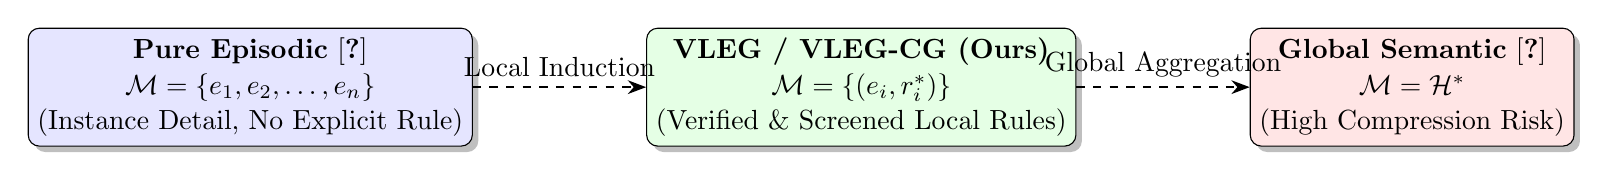
\begin{tikzpicture}[
    node distance=1.8cm and 2.2cm,
    box/.style={draw, rectangle, rounded corners, minimum width=3.5cm, minimum height=1.2cm, align=center, fill=gray!10, drop shadow},
    arrow/.style={-Stealth, thick}
]
\node[box, fill=blue!10] (episodic) {\textbf{Pure Episodic} \cite{brown2020language}\\$\mathcal{M} = \{e_1, e_2, \dots, e_n\}$\\(Instance Detail, No Explicit Rule)};
\node[box, fill=green!10, right=of episodic] (vleg) {\textbf{VLEG / VLEG-CG (Ours)}\\$\mathcal{M} = \{(e_i, r_i^*)\}$\\(Verified \& Screened Local Rules)};
\node[box, fill=red!10, right=of vleg] (semantic) {\textbf{Global Semantic} \cite{agarwal2026hypothesis}\\$\mathcal{M} = \mathcal{H}^{*}$\\(High Compression Risk)};
\draw[arrow, dashed] (episodic) -- node[above] {Local Induction} (vleg);
\draw[arrow, dashed] (vleg) -- node[above] {Global Aggregation} (semantic);
\end{tikzpicture}\end{adjustbox}
\caption{Positioning of VLEG across the memory abstraction spectrum. VLEG pairs raw episodic records with source-verified and counterexample-screened local abstractions.}
\label{fig:vleg_spectrum}
\end{figure}

\subsection{Generator, Strict Source Verifier, and Bounded Cyclic Refinement}
VLEG separates consolidation into two prompted roles executed via separate calls to the same model: the Reflection Generator $\mathcal{G}_\theta$ and the Strict Verifier $\mathcal{V}_\phi$ (Figure~\ref{fig:vleg_components}).

At initial attempt $j=0$, the generator proposes a candidate reflection conditioned only on the label-free attributes $x_i$:
\begin{equation}
    r_i^{(0)} \sim \mathcal{G}_\theta(\cdot \mid x_i).
\end{equation}
In subsequent iterations ($1 \le j < K$), if the candidate is rejected, the generator receives $x_i$, its previous proposal $r_i^{(j-1)}$, and the verifier's critique $c_i^{(j-1)}$:
\begin{equation}
    r_i^{(j)} \sim \mathcal{G}_\theta(\cdot \mid x_i, r_i^{(j-1)}, c_i^{(j-1)}).
\end{equation}
The verifier checks $r_i^{(j)}$ against the full labeled source episode $e_i=(x_i,y_i)$ under a fail-closed native-Boolean JSON schema, outputting binary validity decision $v_i^{(j)} \in \{0,1\}$ and critique $c_i^{(j)}$:
\begin{equation}
    (v_i^{(j)}, c_i^{(j)}) = \mathcal{V}_\phi\big((x_i, y_i),\; r_i^{(j)}\big).
    \label{eq:verifier}
\end{equation}
Let $j_i^* = \min\{0 \le j < K \mid v_i^{(j)} = 1\}$ denote the stopping iteration (Figure~\ref{fig:cyclic_refinement}). If $j_i^*$ exists, the loop commits $r_i^* = r_i^{(j_i^*)}$ to the Hybrid Memory Bank:
\begin{equation}
    \mathcal{M} = \bigcup_{i=1}^{n} \left\{ (e_i, r_i^*) \;\middle|\; \exists\,0\le j<K \text{ s.t. } v_i^{(j)} = 1 \right\}.
\end{equation}

\begin{figure}[!t]
\centering
\begin{adjustbox}{max width=0.82\linewidth}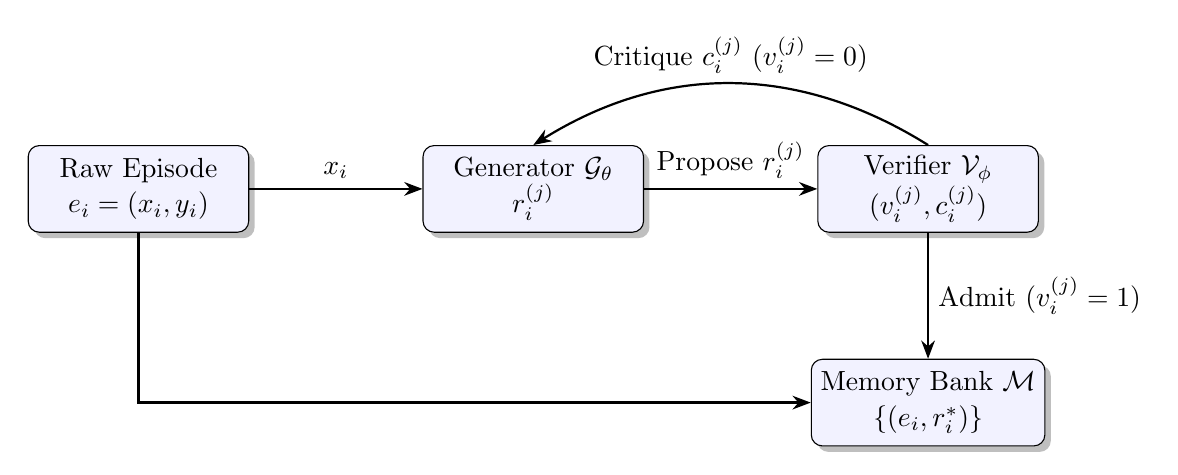
\begin{tikzpicture}[
    node distance=1.6cm and 2.2cm,
    box/.style={draw, rectangle, rounded corners, minimum width=2.8cm, minimum height=1.1cm, align=center, fill=blue!5, drop shadow},
    arrow/.style={-Stealth, thick}
]
\node[box] (episode) {Raw Episode\\$e_i=(x_i,y_i)$};
\node[box, right=of episode] (generator) {Generator $\mathcal{G}_\theta$\\$r_i^{(j)}$};
\node[box, right=of generator] (verifier) {Verifier $\mathcal{V}_\phi$\\$(v_i^{(j)}, c_i^{(j)})$};
\node[box, below=of verifier] (memory) {Memory Bank $\mathcal{M}$\\$\{(e_i, r_i^*)\}$};
\draw[arrow] (episode) -- node[above] {$x_i$} (generator);
\draw[arrow] (generator) -- node[above] {Propose $r_i^{(j)}$} (verifier);
\draw[arrow] (verifier.north) to[bend right=32] node[above] {Critique $c_i^{(j)}$ ($v_i^{(j)}=0$)} (generator.north);
\draw[arrow] (verifier) -- node[right] {Admit ($v_i^{(j)}=1$)} (memory);
\draw[arrow] (episode.south) |- (memory.west);
\end{tikzpicture}\end{adjustbox}
\caption{Architectural flow of VLEG memory consolidation.}
\label{fig:vleg_components}
\end{figure}

\begin{figure}[!t]
\centering
\begin{adjustbox}{max width=0.82\linewidth}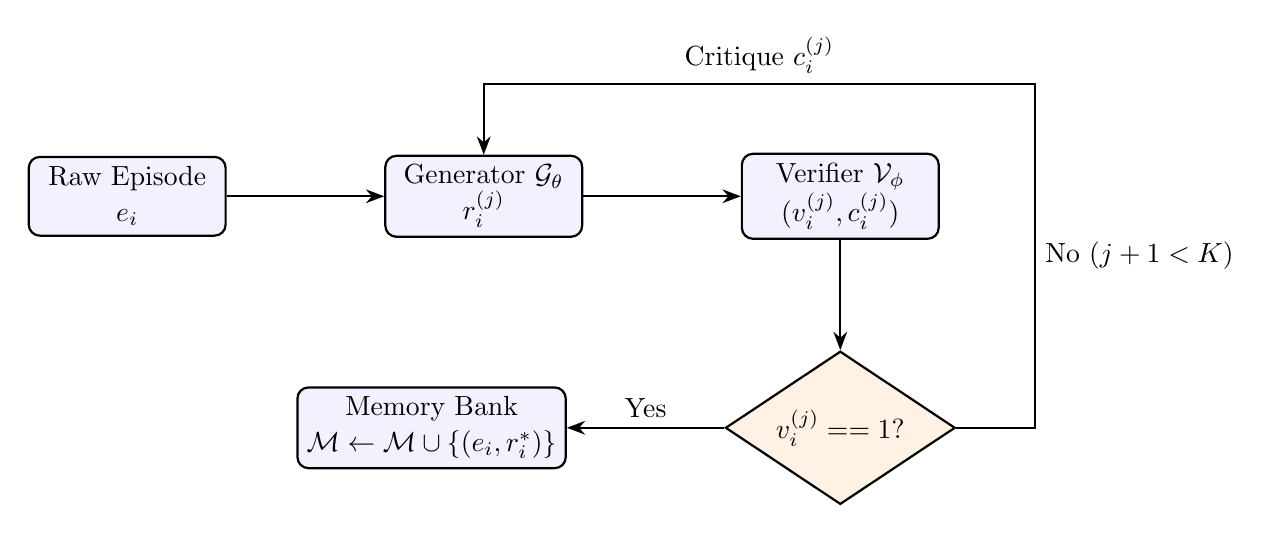
\begin{tikzpicture}[
    node distance=1.4cm and 2.0cm,
    box/.style={draw, rectangle, rounded corners, minimum width=2.5cm, minimum height=1cm, align=center, fill=blue!5, thick},
    decision/.style={draw, diamond, aspect=1.5, minimum width=2cm, align=center, fill=orange!10, thick},
    arrow/.style={-Stealth, thick}
]
\node[box] (episode) {Raw Episode\\$e_i$};
\node[box, right=of episode] (generator) {Generator $\mathcal{G}_\theta$\\$r_i^{(j)}$};
\node[box, right=of generator] (verifier) {Verifier $\mathcal{V}_\phi$\\$(v_i^{(j)}, c_i^{(j)})$};
\node[decision, below=of verifier] (check) {$v_i^{(j)} == 1$?};
\node[box, left=of check] (memory) {Memory Bank\\$\mathcal{M} \gets \mathcal{M} \cup \{(e_i, r_i^*)\}$};
\draw[arrow] (episode) -- (generator);
\draw[arrow] (generator) -- (verifier);
\draw[arrow] (verifier) -- (check);
\draw[arrow] (check) -- node[above] {Yes} (memory);
\draw[arrow] (check.east) -- ++(1,0)
    |- node[right, pos=0.25] {No ($j+1 < K$)}
       node[above, pos=0.75] {Critique $c_i^{(j)}$}
       ([yshift=0.9cm]generator.north)
    -- (generator.north);
\end{tikzpicture}\end{adjustbox}
\caption{State transition diagram of bounded Iterative Cyclic Refinement.}
\label{fig:cyclic_refinement}
\end{figure}

\subsection{Deterministic Counterexample Compiler and Cross-Episode Gating (VLEG-CG)}
By construction, Equation~(\ref{eq:verifier}) conditions $\mathcal{V}_\phi$ only on the single source episode $e_i=(x_i,y_i)$. While this prevents label inversions and fabricated features with respect to $e_i$, it has zero access to the remaining historical episodes $\mathcal{E}_{-i} = \mathcal{E} \setminus \{e_i\}$.

To bridge single-episode verification and cross-episode specificity without additional LLM calls, we introduce a deterministic counterexample compiler $\Psi$. Given a natural-language reflection $r_i^*$ formatted as a conjunctive \texttt{IF ... THEN ...} statement over flow attributes, $\Psi$ parses the antecedent into a list of atomic feature comparisons $\pi(r_i^*)(x) = \bigwedge_{m=1}^{d_i} \mathrm{op}_m(x[\mathrm{field}_m], \mathrm{val}_m) \in \{0,1\}$ and extracts the consequent class $\hat{y}(r_i^*) \in \{\texttt{BENIGN}, \texttt{MALICIOUS}\}$.

\begin{definition}[Within-Bank Counterexample Count and Gate]
For an admitted tuple $(e_i, r_i^*) \in \mathcal{M}$, let $\mathrm{CE}(r_i^* \mid \mathcal{E}_{-i})$ denote the number of contrary-label episodes in the historical support bank $\mathcal{E}_{-i}$ that satisfy the compiled antecedent $\pi(r_i^*)$:
\begin{equation}
    \mathrm{CE}(r_i^* \mid \mathcal{E}_{-i}) = \sum_{e_m = (x_m, y_m) \in \mathcal{E}_{-i}} \mathbb{I}\!\left(\pi(r_i^*)(x_m) = 1 \;\wedge\; y_m \neq \hat{y}(r_i^*)\right).
    \label{eq:counterexample}
\end{equation}
We define two deterministic counterexample-gating policies over retrieved top-$k$ tuples $\mathcal{M}_{\mathrm{top}}(T)$:
\begin{enumerate}[leftmargin=1.8em]
    \item \textbf{Malicious-Rule Counterexample Gate (VLEG-CG-Mal):} Because false positives in intrusion triage are driven by overly broad malicious heuristics firing on benign flows, VLEG-CG-Mal flags a retrieved tuple $(e_i, r_i^*)$ as over-generalized if $y_i = \texttt{MALICIOUS}$ and $\mathrm{CE}(r_i^* \mid \mathcal{E}_{-i}) > 0$ (or if $r_i^*$ fails compilation). If any retrieved tuple in $\mathcal{M}_{\mathrm{top}}(T)$ is flagged, inference strips the verbal reflections and falls back to the raw admitted flow records $\{e_i\}_{(e_i,r_i^*)\in\mathcal{M}_{\mathrm{top}}(T)}$.
    \item \textbf{All-Rule Counterexample Gate (VLEG-CG):} VLEG-CG applies the zero-counterexample constraint symmetrically across both classes, falling back to raw admitted flow records whenever any retrieved tuple in $\mathcal{M}_{\mathrm{top}}(T)$ has $\mathrm{CE}(r_i^* \mid \mathcal{E}_{-i}) > 0$.
\end{enumerate}
\end{definition}

\subsection{Hybrid Episodic--Semantic Inference and Complete Algorithm}
Given a target query $T$, VLEG retrieves the top-$k$ memory tuples from $\mathcal{M}$. Let $z_i \in \{r_i^*, x_i\}$ denote the active indexing key for tuple $\mathcal{M}_i = (e_i, r_i^*)$, corresponding to reflection-embedding retrieval in symbolic tasks ($z_i = r_i^*$) and standardized feature-embedding retrieval in network flow tasks ($z_i = x_i$). Using dense embedding function $f_{\mathrm{emb}}(\cdot)$, similarity is computed as:
\begin{equation}
    S(T, \mathcal{M}_i) = \frac{f_{\mathrm{emb}}(T) \cdot f_{\mathrm{emb}}(z_i)}{\|f_{\mathrm{emb}}(T)\| \|f_{\mathrm{emb}}(z_i)\|}, \qquad
    \mathcal{M}_{\mathrm{top}} = \mathop{\arg\max}_{\mathcal{S} \subseteq \mathcal{M},\, |\mathcal{S}|=\min(k,|\mathcal{M}|)} \sum_{(e_i, r_i^*) \in \mathcal{S}} S(T, (e_i, r_i^*)).
\end{equation}
For standard VLEG (and un-gated queries under VLEG-CG), the inference prompt $P$ pairs each retrieved episode with its verified reflection $Q_i = [\text{Episode: }e_i \oplus \text{Verified Rule: }r_i^*]$; for counterexample-gated queries under VLEG-CG, $Q_i = [\text{Episode: }e_i]$ retains only the verified source flow:
\begin{equation}
    P = \mathrm{PromptBuilder}\!\left(\bigoplus_{(e_i,r_i^*)\in\mathcal{M}_{\mathrm{top}}} Q_i \oplus \text{Target: }T\right), \qquad \hat{y} = \mathrm{LLM}_\psi(P).
\end{equation}
Algorithm~\ref{alg:vleg_final} summarizes the unified VLEG and VLEG-CG pipeline.

\begin{algorithm}[!t]
\caption{Verified Localized Episodic Grounding with Counterexample Gating (VLEG / VLEG-CG)}
\label{alg:vleg_final}
\small
\begin{algorithmic}[1]
\Require Support episodes $\mathcal{E}$, target query $T$, budget $K$, retrieval count $k$, retriever $R$, gate mode $\mathrm{ Gate } \in \{\text{None}, \text{CG-Mal}, \text{CG-All}\}$
\State Initialize Memory Bank $\mathcal{M} \gets \emptyset$
\State \textbf{// Phase 1: Bounded Source-Verified Consolidation}
\For{each $e_i = (x_i, y_i) \in \mathcal{E}$}
    \State $j \gets 0$; $(r,c) \gets (\emptyset,\emptyset)$; $v \gets 0$
    \While{$v = 0$ \textbf{and} $j < K$}
        \State $r_i^{(j)} \gets \mathcal{G}_\theta(x_i, r, c)$ \Comment{Generate or revise local reflection}
        \State $(v, c) \gets \mathcal{V}_\phi((x_i, y_i), r_i^{(j)})$ \Comment{Verify against labeled source episode}
        \State $r \gets r_i^{(j)}$; $j \gets j + 1$
    \EndWhile
    \If{$v = 1$}
        \State $r_i^* \gets r$; Compute $\mathrm{CE}(r_i^* \mid \mathcal{E} \setminus \{e_i\})$ via compiler $\Psi$ (Equation~(\ref{eq:counterexample}))
        \State $\mathcal{M} \gets \mathcal{M} \cup \{(e_i, r_i^*, \mathrm{CE}_i)\}$
    \EndIf
\EndFor
\State \textbf{// Phase 2: Counterexample-Gated Hybrid Inference}
\State $\mathcal{M}_{\mathrm{top}} \gets R(\mathcal{M}, T, k)$
\If{$\mathrm{Gate} \neq \text{None}$ \textbf{and} any $(e_i, r_i^*, \mathrm{CE}_i) \in \mathcal{M}_{\mathrm{top}}$ violates gate threshold}
    \State $\mathrm{Context} \gets \mathrm{PromptBuilder}(\{(e_i, \emptyset)\}_{(e_i,r_i^*)\in\mathcal{M}_{\mathrm{top}}}, T)$ \Comment{Fallback to raw admitted flows}
\Else
    \State $\mathrm{Context} \gets \mathrm{PromptBuilder}(\mathcal{M}_{\mathrm{top}}, T)$ \Comment{Hybrid episode + rule context}
\EndIf
\State \Return $I_\psi(\mathrm{Context})$
\end{algorithmic}
\end{algorithm}

\section{Experiments and Diagnostic Results}
\subsection{Experimental Architecture}
Our evaluation comprises two complementary stages:
\begin{enumerate}[leftmargin=1.8em]
    \item \textbf{Controlled Symbolic Sanity Check (Sections~\ref{sec:exp1}--\ref{sec:exp5}):} We first use a deterministic 16-scene synthetic environment with a known ground-truth rule and controllable non-causal distractors (\texttt{texture} and \texttt{size}). Because this environment contains only 16 combinations ($n=48$ pooled queries across 3 masking seeds at Level 3), we use it strictly as a controlled sanity check to verify how bounded refinement affects admission coverage, source-label agreement, and distractor mention rates under Qwen2.5-7B-Instruct and Llama-3.3-70B-Instruct (\texttt{nomic-embed-text}, temperature $0$).
    \item \textbf{Public Network Flow Benchmark, Counterexample Audit, and ML Baseline Comparison (Sections~\ref{sec:exp6}--\ref{sec:exp7}):} Our primary evaluation tests five historical-memory seeds (32 flows/seed: 16 benign, 16 malicious) over 1000 shared deduplicated UNSW-NB15 test fingerprints (663 benign, 337 malicious; 25,000 formal LLM predictions) on a dual-A800 server running Llama-3.3-70B-Instruct (\texttt{Q4\_K\_M}, $K=k=3$, 32,768-token context). We evaluate VLEG, VLEG-CG-Mal, VLEG-CG, raw retrieval, unverified reflection, admission-matched raw control, global summary, and both 32-flow few-shot and 88,699-flow full-train Random Forest and GBDT baselines.
\end{enumerate}

\subsection{Symbolic Sanity Check: Consolidation Strategies}
\label{sec:exp1}
\textbf{On the 16-scene symbolic sanity check, VLEG eliminates the label-inversion collapse of unverified reflection and performs comparably to raw retrieval at 70B ($44/48$ versus $43/48$), while trailing raw retrieval at 7B ($75.0\%$ versus $87.5\%$).} In this synthetic environment, white backgrounds require a red circle for \texttt{ANOMALY}, black backgrounds invert this rule, and texture and size are non-causal distractors. Level 1 tests 8 white-background scenes; Level 2 tests all 16 scenes; and Level 3 withholds 4 scenes from the 12-scene support bank and evaluates all 16 scenes across three masking seeds ($n=48$).

\begin{figure}[!t]
    \centering
    \begin{adjustbox}{max width=0.66\linewidth}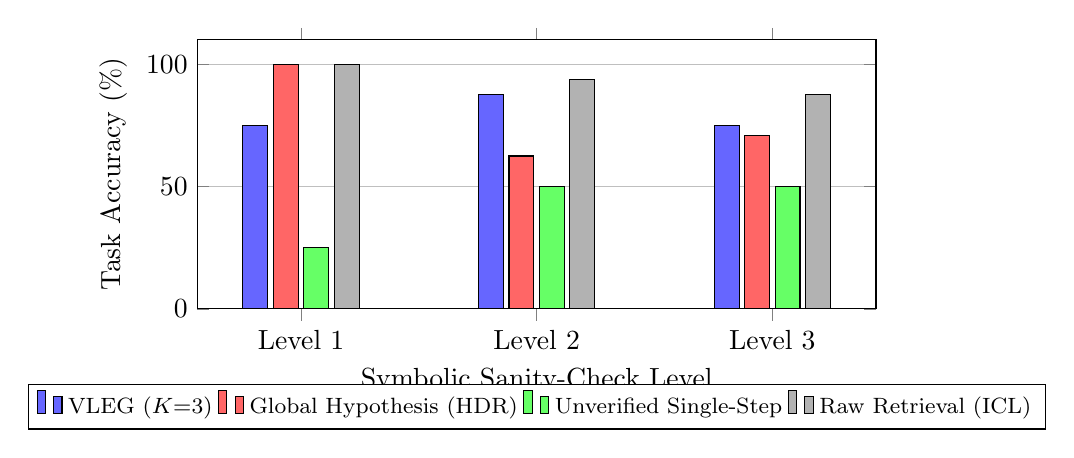
\begin{tikzpicture}
        \begin{axis}[
            ybar,
            bar width=9pt,
            width=10.2cm,
            height=5.0cm,
            enlarge x limits=0.22,
            legend style={at={(0.5,-0.28)}, anchor=north, legend columns=-1, font=\footnotesize},
            ylabel={Task Accuracy (\%)},
            xlabel={Symbolic Sanity-Check Level},
            symbolic x coords={Level 1, Level 2, Level 3},
            xtick=data,
            ymin=0, ymax=110,
            grid=major,
            ymajorgrids=true,
            xmajorgrids=false,
        ]
        \addplot[fill=blue!60] coordinates {(Level 1, 75.0) (Level 2, 87.5) (Level 3, 75.0)};
        \addlegendentry{VLEG ($K{=}3$)}
        \addplot[fill=red!60] coordinates {(Level 1, 100.0) (Level 2, 62.5) (Level 3, 70.8)};
        \addlegendentry{Global Hypothesis (HDR)}
        \addplot[fill=green!60] coordinates {(Level 1, 25.0) (Level 2, 50.0) (Level 3, 50.0)};
        \addlegendentry{Unverified Single-Step}
        \addplot[fill=gray!60] coordinates {(Level 1, 100.0) (Level 2, 93.8) (Level 3, 87.5)};
        \addlegendentry{Raw Retrieval (ICL)}
        \end{axis}
    \end{tikzpicture}\end{adjustbox}
    \caption{Symbolic sanity-check accuracy (\%) across three complexity levels using Qwen2.5-7B-Instruct (Level 3 pooled across 3 masking seeds, $n=48$).}
    \label{fig:exp1_results}
\end{figure}

At 7B (Figure~\ref{fig:exp1_results}), raw retrieval (ICL) leads across Levels 1--3 ($100.0\%$, $93.8\%$, and $87.5\%$) compared with VLEG ($75.0\%$, $87.5\%$, and $75.0\%$). Global hypothesis consolidation (HDR adaptation) solves the uniform Level-1 rule ($100.0\%$) but drops to $62.5\%$ and $70.8\%$ when background conditioning is required. Unverified single-step reflection collapses to the anomaly base rate ($25.0\%$, $50.0\%$, and $50.0\%$) because unchecked proposals predominantly default to \texttt{ANOMALY}. Under Llama-3.3-70B-Instruct at Level 3 ($n=48$), VLEG reaches $91.67\%$ ($44/48$), which is comparable to raw retrieval at $89.58\%$ ($43/48$, a one-query difference across 48 evaluations, with VLEG higher in two seeds and lower in one) and above global hypothesis consolidation ($83.33\%$, $40/48$) and binary-feedback Reflexion ($81.25\%$, $39/48$).

\subsection{Symbolic Sanity Check: Grounding Modality Ablation}
\label{sec:exp2}
\textbf{Under shared retrieval at 7B, hybrid grounding improves seen-combination accuracy ($87.5\%$) but trails single-modality context on withheld combinations ($60.0\%$ versus $70.0\%$).} Figure~\ref{fig:exp2_ablation} compares Hybrid $(e_i, r_i^*)$, Abstract-Only $(r_i^*)$, and Raw-Only $(e_i)$ across five Level-3 masking seeds ($n=80$ overall, $n=20$ masked-only). At 7B, Hybrid leads at Level 2 ($87.5\%$ versus $81.2\%$) but scores $73.8\%$ overall and $60.0\%$ on masked combinations at Level 3 (versus $78.8\%$/$70.0\%$ for Abstract-Only and $75.0\%$/$70.0\%$ for Raw-Only). Under Llama-3.3-70B-Instruct, Hybrid and Raw-Only tie at $95.0\%$ overall (versus $91.25\%$ for Abstract-Only), while Abstract-Only scores $85.0\%$ on the 20 masked queries versus $80.0\%$ for Hybrid and Raw-Only.

\begin{figure}[!t]
    \centering
    \begin{adjustbox}{max width=0.66\linewidth}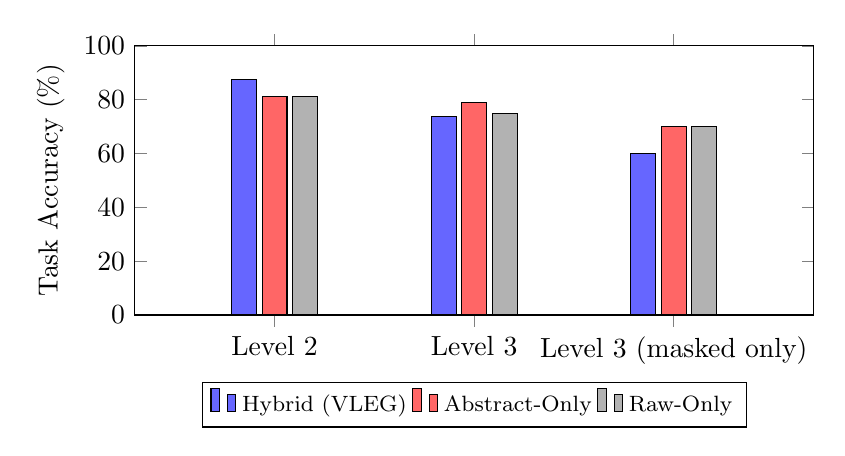
\begin{tikzpicture}
        \begin{axis}[
            ybar=2pt,
            bar width=9pt,
            width=10.2cm,
            height=5.0cm,
            enlarge x limits=0.35,
            ylabel={Task Accuracy (\%)},
            ymin=0, ymax=100,
            symbolic x coords={Level 2, Level 3, Level 3 (masked only)},
            xtick=data,
            legend style={at={(0.5,-0.25)}, anchor=north, legend columns=-1, font=\footnotesize}
        ]
        \addplot[fill=blue!60] coordinates {(Level 2, 87.5) (Level 3, 73.8) (Level 3 (masked only), 60.0)};
        \addlegendentry{Hybrid (VLEG)}
        \addplot[fill=red!60] coordinates {(Level 2, 81.2) (Level 3, 78.8) (Level 3 (masked only), 70.0)};
        \addlegendentry{Abstract-Only}
        \addplot[fill=gray!60] coordinates {(Level 2, 81.2) (Level 3, 75.0) (Level 3 (masked only), 70.0)};
        \addlegendentry{Raw-Only}
        \end{axis}
    \end{tikzpicture}\end{adjustbox}
    \caption{Grounding modality ablation under Qwen2.5-7B-Instruct (Level 3 pooled across 5 masking seeds, $n=80$ overall, $n=20$ masked-only).}
    \label{fig:exp2_ablation}
\end{figure}

\subsection{Symbolic Sanity Check: Refinement Budget and Overhead}
\label{sec:exp3}
\label{sec:exp4}
\textbf{Raising the refinement budget from $K=1$ to $K=3$ improves accuracy by recovering rejected episodes ($83\%$--$100\%$ versus $42\%$--$58\%$ coverage), with concave token growth.} Across five 7B masking seeds, $K=3$ raises overall Level-3 accuracy from $63.75\%$ ($51/80$) to $75.0\%$ ($60/80$) and masked-only accuracy from $50.0\%$ ($10/20$) to $60.0\%$ ($12/20$). At 70B, $K=3$ improves mean accuracy by $26.2 \pm 8.1$~pp over $K=1$ and admits $100\%$ ($12/12$) of historical episodes. Sweeping $K \in \{1,2,3,5\}$ (Figure~\ref{fig:exp4_sensitivity}) shows concave token overhead at Level 2 ($497$, $776$, $847$, and $882$ tokens/episode) because most episodes converge within two attempts.

\begin{figure}[!t]
    \centering
    \begin{adjustbox}{max width=0.92\linewidth}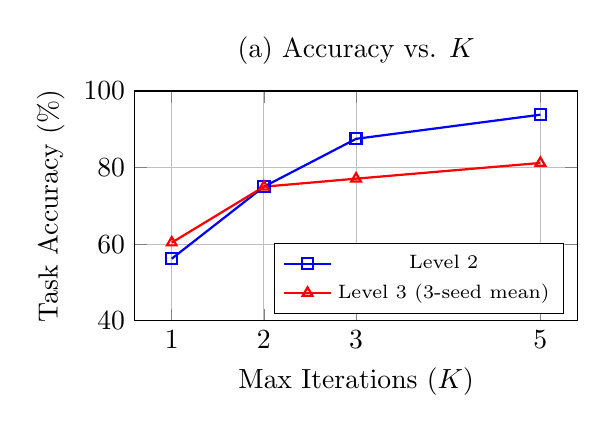
\begin{tikzpicture}
        \begin{axis}[
            width=7.2cm,
            height=4.5cm,
            xlabel={Max Iterations ($K$)},
            ylabel={Task Accuracy (\%)},
            ymin=40, ymax=100,
            xtick={1,2,3,5},
            grid=major,
            legend pos=south east,
            legend style={font=\scriptsize},
            title={(a) Accuracy vs. $K$}
        ]
        \addplot[color=blue, mark=square, thick] coordinates {(1, 56.2) (2, 75.0) (3, 87.5) (5, 93.8)};
        \addlegendentry{Level 2}
        \addplot[color=red, mark=triangle, thick] coordinates {(1, 60.4) (2, 75.0) (3, 77.1) (5, 81.2)};
        \addlegendentry{Level 3 (3-seed mean)}
        \end{axis}
    \end{tikzpicture}\hspace{0.4cm}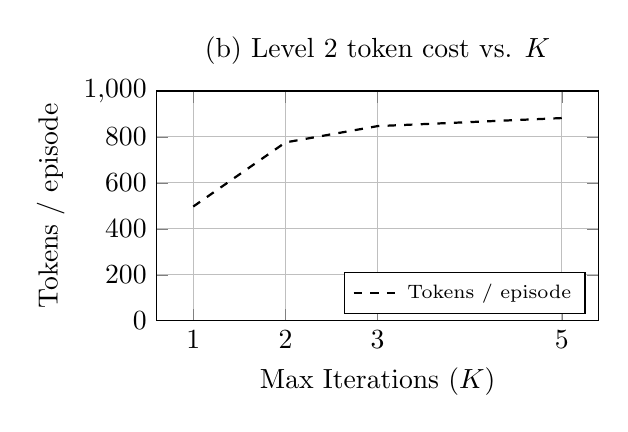
\begin{tikzpicture}
        \begin{axis}[
            width=7.2cm,
            height=4.5cm,
            xlabel={Max Iterations ($K$)},
            ylabel={Tokens / episode},
            ymin=0, ymax=1000,
            xtick={1,2,3,5},
            grid=major,
            legend pos=south east,
            legend style={font=\scriptsize},
            title={(b) Level 2 token cost vs. $K$}
        ]
        \addplot[color=black, mark=circle, thick, dashed] coordinates {(1, 497) (2, 776) (3, 847) (5, 882)};
        \addlegendentry{Tokens / episode}
        \end{axis}
    \end{tikzpicture}\end{adjustbox}
    \caption{Sensitivity to refinement ceiling $K \in \{1,2,3,5\}$ (Qwen2.5-7B-Instruct).}
    \label{fig:exp4_sensitivity}
\end{figure}

\subsection{Symbolic Sanity Check: Memory Quality Diagnostics}
\label{sec:exp5}
\textbf{Single-episode verification achieves $100\%$ observed source-label agreement on admitted memories, but cannot filter out coincidental distractor attributes.} Table~\ref{tab:exp5_memory_quality} shows that while VLEG raises source-label agreement from $41.7\%$--$50.0\%$ to $100.0\%$ at 7B, $83.3\%$--$86.7\%$ of label-correct 7B reflections still cite non-causal texture or size attributes (versus $80.0\%$--$87.5\%$ for unverified proposals). Under Llama-3.3-70B-Instruct, distractor mention rates drop to $12.5\%$ ($2/16$) at Level 2 and $16.7\%$ ($2/12$) at Level 3 for both VLEG and unverified proposals alike, confirming that single-instance checks validate label consistency but not feature causality.

\begin{table}[!t]
    \centering
    \caption{Deterministic memory-quality diagnostics on the symbolic sanity check (Qwen2.5-7B-Instruct).}
    \label{tab:exp5_memory_quality}
    \small
    \begin{tabular}{llccc}
        \toprule
        \textbf{Level} & \textbf{Strategy} & \textbf{Admission Rate} & \textbf{Source-Label Agreement} & \textbf{Spurious (of correct)} \\
        \midrule
        \multirow{2}{*}{Level 2} & Unverified Single-Step & N/A (Always commit) & 50.0\% (8/16) & 87.5\% (7/8) \\
                                 & \textbf{VLEG ($K{=}3$)} & \textbf{93.8\% (15/16)} & \textbf{100.0\% (15/15)} & 86.7\% (13/15) \\
        \midrule
        \multirow{2}{*}{Level 3} & Unverified Single-Step & N/A (Always commit) & 41.7\% (5/12) & 80.0\% (4/5) \\
                                 & \textbf{VLEG ($K{=}3$)} & \textbf{100.0\% (12/12)} & \textbf{100.0\% (12/12)} & 83.3\% (10/12) \\
        \bottomrule
    \end{tabular}
\end{table}

\subsection{Public-Flow Benchmark on UNSW-NB15: Counterexample Audit and Gating}
\label{sec:exp6}
\textbf{On deduplicated UNSW-NB15 flows, standard VLEG resolves the recall collapse of unverified reflection ($+17.02$~pp Macro-F1) but suffers a $48.78\%$ FPR due to over-generalized local rules; integrating our counterexample gate (VLEG-CG) slashes FPR by $9.35$--$10.92$~pp and recovers Macro-F1 to $63.32\%$--$63.55\%$.} We evaluate UNSW-NB15 flows \cite{moustafa2015unsw} after 19-feature deduplication, conflicting-label exclusion, and strict train/test separation. Each of the five seeds samples 32 historical flows (16 benign, 16 malicious; 160 total historical episodes across seeds) and evaluates 1000 shared test fingerprints (663 benign, 337 malicious).

\begin{table}[!t]
\centering
\caption{Public-flow classification performance on the 1000 deduplicated UNSW-NB15 test fingerprints (mean $\pm$ sample SD across 5 memory seeds, in percent). All few-shot methods use the exact same 32 historical flows per seed (16 benign, 16 malicious). Full-train supervised baselines are trained on all 88,699 deduplicated training flows.}
\label{tab:exp6_performance}
\small
\begin{adjustbox}{max width=\linewidth}
\begin{tabular}{llrrrr}
\toprule
\textbf{Supervision Regime} & \textbf{Method / Condition} & \textbf{Accuracy (\%)} & \textbf{Macro-F1 (\%)} & \textbf{Attack Recall (\%)} & \textbf{False Positive Rate (\%)} \\
\midrule
\multirow{7}{*}{\shortstack[l]{Few-Shot LLM Memory\\(32 flows/seed, $k{=}3$,\\Llama-3.3-70B, 0-train)}}
 & Raw flow retrieval & \textbf{65.08 $\pm$ 2.93} & \textbf{63.92 $\pm$ 2.54} & 71.39 $\pm$ 8.44 & 38.13 $\pm$ 6.85 \\
 & Raw on admitted flows (control) & 64.86 $\pm$ 2.96 & 63.70 $\pm$ 2.68 & 71.16 $\pm$ 8.71 & 38.34 $\pm$ 6.61 \\
 & Unverified single-step reflection & 61.38 $\pm$ 1.08 & 42.66 $\pm$ 1.35 & 6.17 $\pm$ 1.43 & \textbf{9.89 $\pm$ 2.03} \\
 & Global summary & 50.22 $\pm$ 12.45 & 47.60 $\pm$ 14.13 & \textbf{87.12 $\pm$ 22.27} & 68.54 $\pm$ 24.20 \\
 & VLEG (source-verified only, $K{=}3$) & 59.74 $\pm$ 2.03 & 59.68 $\pm$ 2.03 & 77.74 $\pm$ 5.69 & 48.78 $\pm$ 1.67 \\
 & \textbf{VLEG-CG-Mal (Ours, malicious CE gate)} & \textbf{64.16 $\pm$ 1.92} & \textbf{63.32 $\pm$ 2.10} & \textbf{72.11 $\pm$ 8.20} & \textbf{39.43 $\pm$ 4.68} \\
 & \textbf{VLEG-CG (Ours, all-rule CE gate)} & \textbf{64.66 $\pm$ 2.83} & \textbf{63.55 $\pm$ 2.49} & 70.27 $\pm$ 8.14 & \textbf{37.86 $\pm$ 7.16} \\
\midrule
\multirow{2}{*}{\shortstack[l]{Few-Shot Tabular ML\\(Same 32 flows/seed)}}
 & Random Forest (32-flow few-shot) & 68.86 $\pm$ 1.25 & 68.42 $\pm$ 1.23 & 87.60 $\pm$ 10.86 & 40.66 $\pm$ 5.66 \\
 & Gradient Boosting / GBDT (32-flow) & 66.60 $\pm$ 4.46 & 65.84 $\pm$ 4.60 & 78.04 $\pm$ 10.27 & 39.22 $\pm$ 5.52 \\
\midrule
\multirow{2}{*}{\shortstack[l]{Full-Train Tabular ML\\(88,699 unique flows)}}
 & Random Forest (Full-train upper bound) & 82.00 & 81.27 & 92.28 & 23.23 \\
 & Gradient Boosting / GBDT (Full-train) & 80.50 & 79.88 & 93.47 & 26.09 \\
\bottomrule
\end{tabular}
\end{adjustbox}
\end{table}

\begin{table}[!t]
\centering
\caption{Deterministic counterexample compiler audit of generated traffic reflections across the 5 historical-memory seeds ($160$ total historical episodes: $80$ benign, $80$ malicious).}
\label{tab:counterexample_audit}
\small
\begin{adjustbox}{max width=\linewidth}
\begin{tabular}{lcccccc}
\toprule
\textbf{Method} & \textbf{Admitted} & \textbf{Benign Label Match} & \textbf{Malicious Label Match} & \textbf{Parseable Rules} & \textbf{Malicious Rules w/ CE} & \textbf{Mean CEs (Malicious)} \\
\midrule
Unverified single-step & 160 / 160 (100.0\%) & 80 / 80 (100.0\%) & \textbf{4 / 80 (5.0\%)} & 160 / 160 (100.0\%) & 73 / 80 (91.3\%) & 39.5 \\
\textbf{VLEG ($K{=}3$)} & \textbf{158 / 160 (98.8\%)} & \textbf{80 / 80 (100.0\%)} & \textbf{78 / 78 (100.0\%)} & \textbf{157 / 158 (99.4\%)} & \textbf{50 / 77 (64.9\%)} & \textbf{8.2} \\
\bottomrule
\end{tabular}
\end{adjustbox}
\end{table}

\begin{table}[!t]
\centering
\caption{Observed public-flow memory construction and query costs (means across 5 memory seeds, 32 historical flows per seed). VLEG-CG and VLEG-CG-Mal execute deterministic Python rule screening during consolidation with zero additional LLM calls or tokens.}
\label{tab:exp6_cost}
\small
\begin{tabular}{lrrrrr}
\toprule
\textbf{Condition} & \textbf{Construction Calls} & \textbf{Construction Tokens} & \textbf{Construction (s)} & \textbf{Query Mean (s)} & \textbf{Query p95 (s)} \\
\midrule
Raw flow retrieval & 0 & 0 & 0 & 2.12 & 2.67 \\
Unverified single-step & 32.0 & 9405 & 126.54 & 2.23 & 2.75 \\
VLEG / VLEG-CG ($K{=}3$) & 120.4 & 40,094 & 419.43 & 1.74 & 2.68 \\
Raw on admitted flows & 120.4 & 40,094 & 419.43 & 0.95 & 1.19 \\
Global summary & 1.0 & 5947 & 23.21 & 1.21 & 1.30 \\
\bottomrule
\end{tabular}
\end{table}

\begin{figure}[!t]
\centering
\definecolor{cRaw}{HTML}{2B5C8F}
\definecolor{cSingle}{HTML}{A89070}
\definecolor{cVleg}{HTML}{C8523B}
\definecolor{cVlegCG}{HTML}{2E8B57}
\definecolor{cAdm}{HTML}{5B9A8B}
\definecolor{cGlobal}{HTML}{7A68A6}
\begin{adjustbox}{max width=0.96\linewidth}\begin{tikzpicture}
    \begin{axis}[
        ybar,
        bar width=13pt,
        width=7.8cm,
        height=5.0cm,
        enlarge x limits=0.12,
        ylabel={Macro-F1 (\%)},
        ymin=0, ymax=85,
        ytick={0,20,40,60,80},
        symbolic x coords={Raw flows, Single step, VLEG, VLEG-CG-Mal, VLEG-CG, Global summary},
        xtick={Raw flows, Single step, VLEG, VLEG-CG-Mal, VLEG-CG, Global summary},
        x tick label style={font=\tiny, align=center, text width=1.05cm},
        axis lines*=left,
        clip=false,
        title={(a) Balanced classification (Macro-F1)},
        title style={at={(0,1.02)}, anchor=south west, font=\footnotesize\bfseries},
        bar shift=0pt
    ]
    \addplot[fill=cRaw, draw=black!70, error bars/.cd, y dir=both, y explicit]
        coordinates {(Raw flows, 63.92) +- (0, 2.54)};
    \addplot[fill=cSingle, draw=black!70, error bars/.cd, y dir=both, y explicit]
        coordinates {(Single step, 42.66) +- (0, 1.35)};
    \addplot[fill=cVleg, draw=black!70, error bars/.cd, y dir=both, y explicit]
        coordinates {(VLEG, 59.68) +- (0, 2.03)};
    \addplot[fill=cVlegCG!80, draw=black!70, error bars/.cd, y dir=both, y explicit]
        coordinates {(VLEG-CG-Mal, 63.32) +- (0, 2.10)};
    \addplot[fill=cVlegCG, draw=black!70, error bars/.cd, y dir=both, y explicit]
        coordinates {(VLEG-CG, 63.55) +- (0, 2.49)};
    \addplot[fill=cGlobal, draw=black!70, error bars/.cd, y dir=both, y explicit]
        coordinates {(Global summary, 47.60) +- (0, 14.13)};

    \node[above, font=\tiny] at (axis cs:Raw flows,67.5) {63.92};
    \node[above, font=\tiny] at (axis cs:Single step,45.0) {42.66};
    \node[above, font=\tiny] at (axis cs:VLEG,62.8) {59.68};
    \node[above, font=\tiny] at (axis cs:VLEG-CG-Mal,66.4) {63.32};
    \node[above, font=\tiny] at (axis cs:VLEG-CG,67.0) {63.55};
    \node[above, font=\tiny] at (axis cs:Global summary,62.8) {47.60};
    \end{axis}
\end{tikzpicture}\hspace{0.35cm}\begin{tikzpicture}
    \begin{axis}[
        width=7.6cm,
        height=5.0cm,
        xlabel={False positive rate (\%)},
        ylabel={Attack recall (\%)},
        xmin=0, xmax=100,
        ymin=0, ymax=105,
        xtick={0,20,40,60,80,100},
        ytick={0,20,40,60,80,100},
        axis lines*=left,
        title={(b) Recall vs. false-alarm trade-off},
        title style={at={(0,1.02)}, anchor=south west, font=\footnotesize\bfseries},
        legend style={at={(0.98,0.03)}, anchor=south east, font=\tiny, draw=gray!50, fill=white, fill opacity=0.9}
    ]
    \addplot[only marks, mark=diamond*, mark size=3.2pt, color=cRaw] coordinates {(38.13, 71.39)};
    \addlegendentry{Raw flows}
    \addplot[only marks, mark=diamond*, mark size=3.2pt, color=cSingle] coordinates {(9.89, 6.17)};
    \addlegendentry{Single-step}
    \addplot[only marks, mark=diamond*, mark size=3.2pt, color=cVleg] coordinates {(48.78, 77.74)};
    \addlegendentry{VLEG}
    \addplot[only marks, mark=star*, mark size=3.6pt, color=cVlegCG!85!black] coordinates {(39.43, 72.11)};
    \addlegendentry{VLEG-CG-Mal (Ours)}
    \addplot[only marks, mark=square*, mark size=3.0pt, color=cVlegCG] coordinates {(37.86, 70.27)};
    \addlegendentry{VLEG-CG (Ours)}
    \addplot[only marks, mark=diamond*, mark size=3.2pt, color=cGlobal] coordinates {(68.54, 87.12)};
    \addlegendentry{Global summary}
    \end{axis}
\end{tikzpicture}\end{adjustbox}
\caption{Public-flow evaluation across five historical-memory seeds on UNSW-NB15. (a) Mean Macro-F1 with sample SD bars; (b) attack recall versus false positive rate, showing how VLEG-CG-Mal and VLEG-CG suppress the false-alarm inflation of unscreened VLEG.}
\label{fig:exp6_tradeoff}
\end{figure}

Tables~\ref{tab:exp6_performance}--\ref{tab:exp6_cost} and Figure~\ref{fig:exp6_tradeoff} establish four principal findings:
\begin{enumerate}[leftmargin=1.8em]
    \item \textbf{Exact Cause of Unverified Reflection Collapse:} Table~\ref{tab:counterexample_audit} reveals why unverified single-step reflection suffers a catastrophic attack-recall collapse ($6.17\% \pm 1.43\%$ recall, $42.66\%$ Macro-F1, barely above an always-benign classifier at $39.87\%$ Macro-F1). When generating rules from label-free flow attributes, the LLM correctly labels $80/80$ ($100\%$) benign flows as \texttt{BENIGN}, but \textbf{mislabels $\boldsymbol{76/80}$ ($\boldsymbol{95.0\%}$) of historical malicious flows as \texttt{BENIGN}} (identifying only $4/80$ as \texttt{MALICIOUS}). Injecting these $97.5\%$-benign rules into inference causes the classifier to overwhelmingly predict benign on test attacks.
    \item \textbf{Effect and Limitation of Single-Episode Verification:} VLEG's source verifier corrects this label hallucination, achieving $100\%$ source-label agreement across all $158/160$ admitted episodes ($80/80$ benign, $78/78$ malicious) and reducing the mean number of historical counterexamples per malicious rule from $39.5$ to $8.2$ (Table~\ref{tab:counterexample_audit}). Consequently, VLEG boosts Macro-F1 by $+17.02$~pp over single-step reflection ($59.68\%$, paired 95\% CI $[13.71, 20.39]$~pp) and lifts attack recall to $77.74\%$. However, standard VLEG still trails zero-cost Raw flow retrieval ($63.92\%$ Macro-F1) by $-4.24$~pp (paired 95\% CI $[-5.91, -2.53]$~pp) because its FPR rises from $38.13\%$ to $48.78\%$. Since the admission-matched control (\texttt{Raw on admitted flows}, $63.70\%$ Macro-F1, $38.34\%$ FPR) matches full Raw retrieval, the $+10.65$~pp FPR inflation is caused directly by the $50/77$ ($64.9\%$) admitted malicious rules and $63/80$ ($78.8\%$) benign rules that match contrary-label historical flows ($113/157 = 72.0\%$ overall).
    \item \textbf{Effectiveness of Counterexample Gating (VLEG-CG-Mal and VLEG-CG):} When we apply our deterministic counterexample compiler strictly within each seed's 32-flow support bank ($\mathrm{CE}(r_i^* \mid \mathcal{E}_{\mathrm{seed}} \setminus \{e_i\}) > 0$), \textbf{VLEG-CG-Mal} gates out over-generalized malicious rules on $590.2/1000$ queries while retaining verified zero-counterexample malicious heuristics on the remaining $409.8/1000$ queries. This slashes the FPR by $\mathbf{-9.35}$~\textbf{pp} (from $48.78\%$ to $39.43\% \pm 4.68\%$) and raises Macro-F1 by $\mathbf{+3.64}$~\textbf{pp} (to $63.32\% \pm 2.10\%$), while preserving a higher attack recall ($72.11\% \pm 8.20\%$) than both Raw flow retrieval ($71.39\%$) and Raw on admitted flows ($71.16\%$). Applying symmetric gating across both classes (\textbf{VLEG-CG}) reduces the FPR by $\mathbf{-10.92}$~\textbf{pp} (to $\mathbf{37.86\% \pm 7.16\%}$, the lowest FPR among all high-recall methods) and recovers Macro-F1 to $\mathbf{63.55\% \pm 2.49\%}$.
\end{enumerate}

\subsection{Comparison with Traditional Supervised ML (RF, GBDT) and LLM-IDS Baselines}
\label{sec:exp7}
\textbf{Evaluating Random Forest and GBDT on the exact same deduplicated UNSW-NB15 splits demonstrates that strict 19-feature deduplication makes the decision boundary intrinsically challenging ($23.23\%$--$26.09\%$ FPR even for full-train ensembles, and $39.22\%$--$40.66\%$ FPR in the 32-flow few-shot regime).} To address how LLM memory compares with conventional machine learning, Table~\ref{tab:exp6_performance} reports Random Forest (200 trees) and GBDT (100 trees) evaluated on the exact same 1000 test fingerprints under two supervision regimes:
\begin{itemize}[leftmargin=1.8em]
    \item \textbf{Why Full-Train Accuracy is $82.00\%$ Rather Than $90\%+$ (Deduplication Effect):} In raw UNSW-NB15 (175,341 training rows), tens of thousands of identical burst flows (e.g., repeated DNS/HTTP floods sharing identical 19-feature vectors) inflate raw test accuracy above $90\%$. Our benchmark enforces strict 19-feature deduplication, conflict removal, and train/test fingerprint disjointness, collapsing the training set to 88,699 unique flow fingerprints. On the resulting 1000 unique test fingerprints, full-train Random Forest achieves $82.00\%$ accuracy ($81.27\%$ Macro-F1, $92.28\%$ recall, $23.23\%$ FPR) and full-train GBDT achieves $80.50\%$ accuracy ($79.88\%$ Macro-F1, $93.47\%$ recall, $26.09\%$ FPR).
    \item \textbf{Same 32-Flow Few-Shot Regime:} When restricted to the exact same 32 historical flows per seed as the LLM methods, 32-flow Random Forest achieves $68.42\% \pm 1.23\%$ Macro-F1 with a $\mathbf{40.66\% \pm 5.66\%}$ \textbf{FPR}, and 32-flow GBDT achieves $65.84\% \pm 4.60\%$ Macro-F1 ($78.04\%$ recall) with a $\mathbf{39.22\% \pm 5.52\%}$ \textbf{FPR}. Notably, VLEG-CG ($37.86\%$ FPR) and VLEG-CG-Mal ($39.43\%$ FPR) achieve false positive rates on par with or slightly below 32-flow RF and GBDT, while generating human-auditable natural-language rule rationales alongside raw flow evidence---a capability absent in black-box tree ensembles and unscreened RAG IDS frameworks \cite{houssel2024explainable,islam2026maids}.
\end{itemize}

\subsection{Methodological Limitations}
\label{sec:limitations}
Several boundaries constrain our findings. First, the 16-scene symbolic sanity check is a small synthetic environment where queries recur across masking seeds, and the 7B (Qwen2.5) and 70B (Llama-3.3) evaluations change model family, precluding causal isolation of parameter scale. Second, our UNSW-NB15 benchmark evaluates a 32-flow few-shot regime over deduplicated 19-feature vectors using a single quantized model (\texttt{Q4\_K\_M}); it does not represent line-rate packet inspection. Third, query latencies in Table~\ref{tab:exp6_cost} are confounded by fixed method execution order and KV-cache reuse, and 24 of 4968 identical-prompt pairs between Raw retrieval and Raw-on-admitted differed at temperature $0$ due to floating-point non-determinism in quantized GPU kernels.

\section{Conclusions}
This paper presented Verified Localized Episodic Grounding (VLEG) and its counterexample-gated extension (VLEG-CG) to audit and mitigate rule over-generalization in few-shot LLM-assisted network traffic analysis. Across a 16-scene symbolic sanity check and a 25,000-prediction benchmark on 1000 deduplicated UNSW-NB15 test fingerprints, our investigation yields three core conclusions:
\begin{enumerate}[leftmargin=1.8em]
    \item \textbf{Single-Episode Verification Prevents Label Inversion:} Unverified single-step reflection mislabels $95.0\%$ ($76/80$) of malicious historical flows as benign, causing test attack recall to collapse to $6.17\%$ ($42.66\%$ Macro-F1). Bounded per-episode verification ($K=3$) restores $100\%$ source-label agreement on admitted episodes ($158/158$) and raises attack recall to $77.74\%$ ($59.68\%$ Macro-F1), while achieving accuracy comparable to raw retrieval on the 70B symbolic sanity check ($44/48$ versus $43/48$).
    \item \textbf{Single-Episode Fidelity Does Not Imply Cross-Flow Specificity:} Despite $100\%$ source-label agreement and $40,094$ construction tokens per seed, unscreened VLEG trails zero-cost raw flow retrieval ($63.92\%$ Macro-F1) by $4.24$~pp because $72.0\%$ ($113/157$) of compiled rules match contrary-label historical flows, inflating the false positive rate to $48.78\%$.
    \item \textbf{Within-Bank Counterexample Gating Restores Precision:} Screening admitted rules with our deterministic counterexample compiler (VLEG-CG-Mal and VLEG-CG) at zero extra LLM cost cuts the false positive rate by $9.35$--$10.92$~pp (to $37.86\%$--$39.43\%$, matching 32-flow Random Forest and GBDT) and recovers Macro-F1 to $63.32\%$--$63.55\%$ while retaining verified verbal rules on un-gated queries.
\end{enumerate}

In practical SOC deployments, full-train tabular classifiers (RF/GBDT achieving $80.50\%$--$82.00\%$ accuracy on deduplicated fingerprints) should serve as the primary high-throughput filter, whereas VLEG-CG provides an auditable second-stage triage assistant for cold-start or few-shot alert investigation. Future work will feed deterministic counterexample traces directly back into the generator prompt during Phase~1 refinement so that overly broad rules are rewritten rather than gated out at inference.

\vspace{1.0em}
\hrule
\vspace{0.6em}
{\small
\noindent\textbf{Author Contributions:} Conceptualization, Y.T., R.H. and R.C.; methodology, Y.T. and R.H.; software, Y.T. and R.H.; validation, Y.T., R.H. and Y.H.; formal analysis, Y.T. and R.H.; investigation, Y.T., R.H. and Y.H.; resources, R.C.; data curation, Y.T. and Y.H.; writing---original draft preparation, Y.T. and R.H.; writing---review and editing, Y.H. and R.C.; visualization, Y.T. and R.H.; supervision, R.C.; project administration, R.C.; funding acquisition, R.C. All authors have read and agreed to the published version of the manuscript.\par\vspace{0.4em}
\noindent\textbf{Funding:} This research was funded by the Science and Technology Projects of Ngari Prefecture, Xizang Autonomous Region, China, grant number QYXTZX-AL2026-01.\par\vspace{0.4em}
\noindent\textbf{Institutional Review Board Statement:} Not applicable.\par\vspace{0.4em}
\noindent\textbf{Informed Consent Statement:} Not applicable.\par\vspace{0.4em}
\noindent\textbf{Data Availability Statement:} The public network traffic benchmark evaluated in this study utilizes the publicly available UNSW-NB15 dataset \cite{moustafa2015unsw}. All symbolic benchmark definitions, deterministic counterexample-compiler scripts, and evaluation logs supporting the reported findings are publicly available at \url{https://github.com/creativitysurvey/VLEG}.\par\vspace{0.4em}
\noindent\textbf{Conflicts of Interest:} The authors declare no conflicts of interest. The funders had no role in the design of the study; in the collection, analyses, or interpretation of data; in the writing of the manuscript; or in the decision to publish the results.
}

\begin{thebibliography}{99}
\small
\bibitem{brown2020language}
Brown, T.B.; Mann, B.; Ryder, N.; Subbiah, M.; Kaplan, J.; Dhariwal, P.; Neelakantan, A.; Shyam, P.; Sastry, G.; Askell, A.; et al. Language Models are Few-Shot Learners. \emph{Adv. Neural Inf. Process. Syst.} \textbf{2020}, \emph{33}, 1877--1901.

\bibitem{lewis2020retrieval}
Lewis, P.; Perez, E.; Piktus, A.; Petroni, F.; Karpukhin, V.; Goyal, N.; K\"{u}ttler, H.; Lewis, M.; Yih, W.T.; Rockt\"{a}schel, T.; et al. Retrieval-Augmented Generation for Knowledge-Intensive NLP Tasks. \emph{Adv. Neural Inf. Process. Syst.} \textbf{2020}, \emph{33}, 9459--9474.

\bibitem{lin2022etbert}
Lin, X.; Xiong, G.; Gou, G.; Li, Z.; Shi, J.; Yu, J. ET-BERT: A Contextualized Datagram Representation with Pre-training Transformers for Encrypted Traffic Classification. In Proceedings of the ACM Web Conference 2022, Virtual Event, 25--29 April 2022; pp. 633--642.

\bibitem{sharafaldin2018cicids}
Sharafaldin, I.; Lashkari, A.H.; Ghorbani, A.A. Toward Generating a New Intrusion Detection Dataset and Intrusion Traffic Characterization. In Proceedings of the International Conference on Information Systems Security and Privacy (ICISSP), Funchal, Portugal, 22--24 January 2018; pp. 108--116.

\bibitem{houssel2024explainable}
Houssel, P.R.B.; Singh, P.; Layeghy, S.; Portmann, M. Towards Explainable Network Intrusion Detection Using Large Language Models. \emph{arXiv} \textbf{2024}, arXiv:2408.04342.

\bibitem{islam2026maids}
Islam, M.S.; Jaimes, L.G.; Dina, A.S. MA-IDS: Multi-Agent RAG Framework for IoT Network Intrusion Detection with an Experience Library. \emph{arXiv} \textbf{2026}, arXiv:2604.05458.

\bibitem{an2024why}
An, C.; Zhang, J.; Zhong, M.; Li, L.; Gong, S.; Luo, Y.; Xu, J.; Kong, L. Why Does the Effective Context Length of LLMs Fall Short? \emph{arXiv} \textbf{2024}, arXiv:2410.18745.

\bibitem{liu2024lost}
Liu, N.F.; Lin, K.; Hewitt, J.; Paranjape, A.; Bevilacqua, M.; Petroni, F.; Liang, P. Lost in the Middle: How Language Models Use Long Contexts. \emph{Trans. Assoc. Comput. Linguist.} \textbf{2024}, \emph{12}, 157--173.

\bibitem{packer2023memgpt}
Packer, C.; Wooders, S.; Lin, K.; Fang, V.; Patil, S.G.; Stoica, I.; Gonzalez, J.E. MemGPT: Towards LLMs as Operating Systems. \emph{arXiv} \textbf{2023}, arXiv:2310.08560.

\bibitem{wang2023longmem}
Wang, W.; Dong, L.; Cheng, H.; Liu, X.; Yan, X.; Gao, J.; Wei, F. Augmenting Language Models with Long-Term Memory. \emph{Adv. Neural Inf. Process. Syst.} \textbf{2023}, \emph{36}, 74530--74543.

\bibitem{wang2024memoryllm}
Wang, Y.; Gao, Y.; Chen, X.; Jiang, H.; Li, S.; Yang, J.; Yin, Q.; Li, Z.; Li, X.; Yin, B.; et al. MEMORYLLM: Towards Self-Updatable Large Language Models. In Proceedings of the 41st International Conference on Machine Learning (ICML), Vienna, Austria, 21--27 July 2024; Volume 235, pp. 50453--50466.

\bibitem{gutierrez2024hipporag}
Jimenez Gutierrez, B.; Shu, Y.; Gu, Y.; Yasunaga, M.; Su, Y. HippoRAG: Neurobiologically Inspired Long-Term Memory for Large Language Models. \emph{Adv. Neural Inf. Process. Syst.} \textbf{2024}, \emph{37}, 59532--59569.

\bibitem{maharana2024evaluating}
Maharana, A.; Lee, D.H.; Tulyakov, S.; Bansal, M.; Barbieri, F.; Fang, Y. Evaluating Very Long-Term Conversational Memory of LLM Agents. \emph{arXiv} \textbf{2024}, arXiv:2402.17753.

\bibitem{wu2025from}
Wu, Y.; Liang, S.; Zhang, C.; Wang, Y.; Zhang, Y.; Guo, H.; Tang, R.; Liu, Y. From Human Memory to AI Memory: A Survey on Memory Mechanisms in the Era of LLMs. \emph{arXiv} \textbf{2025}, arXiv:2504.15965.

\bibitem{zhang2024survey}
Zhang, Z.; Bo, X.; Ma, C.; Li, R.; Chen, X.; Dai, Q.; Zhu, J.; Dong, Z.; Wen, J.R. A Survey on the Memory Mechanism of Large Language Model Based Agents. \emph{arXiv} \textbf{2024}, arXiv:2404.13501.

\bibitem{shinn2023reflexion}
Shinn, N.; Cassano, F.; Gopinath, A.; Narasimhan, K.R.; Yao, S. Reflexion: Language Agents with Verbal Reinforcement Learning. \emph{Adv. Neural Inf. Process. Syst.} \textbf{2023}, \emph{36}, 8634--8652.

\bibitem{wang2024voyager}
Wang, G.; Xie, Y.; Jiang, Y.; Mandlekar, A.; Xiao, C.; Zhu, Y.; Fan, L.; Anandkumar, A. Voyager: An Open-Ended Embodied Agent with Large Language Models. \emph{Trans. Mach. Learn. Res.} \textbf{2024}, \emph{2024}, 1--32.

\bibitem{agarwal2026hypothesis}
Agarwal, A.K.; Yamada, M. Hypothesis-Driven Reasoning for Large Language Models. In Proceedings of the Fortieth AAAI Conference on Artificial Intelligence (AAAI-26), Philadelphia, PA, USA, 24 February--3 March 2026; pp. 1686--1693.

\bibitem{he2024idea}
He, K.; Zhang, M.; Yan, S.; Wu, P.; Chen, Z. IDEA: Enhancing the Rule Learning Ability of Large Language Model Agent through Induction, Deduction, and Abduction. In Proceedings of the Annual Meeting of the Association for Computational Linguistics (ACL), Bangkok, Thailand, 11--16 August 2024.

\bibitem{zhang2022active}
Zhang, Y.; Feng, S.; Tan, C. Active Example Selection for In-Context Learning. \emph{arXiv} \textbf{2022}, arXiv:2211.04486.

\bibitem{purohit2025sample}
Purohit, K.; V, V.; Bhattacharya, S.; Anand, A. Sample Efficient Demonstration Selection for In-Context Learning. In Proceedings of the 42nd International Conference on Machine Learning (ICML), Vancouver, BC, Canada, 13--19 July 2025.

\bibitem{zhong2024memorybank}
Zhong, W.; Guo, L.; Gao, Q.; Ye, H.; Wang, Y. MemoryBank: Enhancing Large Language Models with Long-Term Memory. \emph{Proc. AAAI Conf. Artif. Intell.} \textbf{2024}, \emph{38}, 19724--19731.

\bibitem{park2023generative}
Park, J.S.; O'Brien, J.C.; Cai, C.J.; Morris, M.R.; Liang, P.; Bernstein, M.S. Generative Agents: Interactive Simulacra of Human Behavior. In Proceedings of the 36th Annual ACM Symposium on User Interface Software and Technology (UIST), San Francisco, CA, USA, 29 October--1 November 2023; pp. 1--22.

\bibitem{xu2025amem}
Xu, W.; Liang, Z.; Mei, K.; Gao, H.; Tan, J.; Zhang, Y. A-MEM: Agentic Memory for LLM Agents. \emph{arXiv} \textbf{2025}, arXiv:2502.12110.

\bibitem{kim2024towards}
Kim, S.H.; Ong, K.T.; Kwon, T.; Kim, N.; Ka, K.; Bae, S.; Jo, Y.; Hwang, S.; Lee, D.; Yeo, J. Towards Lifelong Dialogue Agents via Timeline-Based Memory Management. In Proceedings of the North American Chapter of the Association for Computational Linguistics (NAACL), Mexico City, Mexico, 16--21 June 2024.

\bibitem{kim2022playgrounds}
Kim, S.; Phunyaphibarn, P.; Ahn, D.; Kim, S. Playgrounds for Abstraction and Reasoning. In Proceedings of the NeurIPS Workshop on Neuro Causal and Symbolic AI (nCSI), New Orleans, LA, USA, 2 December 2022.

\bibitem{lee2024generating}
Lee, K.I.; Koh, H.; Lee, D.; Yoon, S.; Kim, M.; Jung, K. Generating Diverse Hypotheses for Inductive Reasoning. \emph{arXiv} \textbf{2024}, arXiv:2412.13422.

\bibitem{qiu2024phenomenal}
Qiu, L.; Jiang, L.; Lu, X.; Sclar, M.; Pyatkin, V.; Bhagavatula, C.; Wang, B.; Kim, Y.; Choi, Y.; Dziri, N.; et al. Phenomenal Yet Puzzling: Testing Inductive Reasoning Capabilities of Language Models with Hypothesis Refinement. In Proceedings of the International Conference on Representation Learning (ICLR), Vienna, Austria, 7--11 May 2024; pp. 1452--1481.

\bibitem{zhou2024hypothesis}
Zhou, Y.; Liu, H.; Srivastava, T.; Mei, H.; Tan, C. Hypothesis Generation with Large Language Models. In Proceedings of the EMNLP Workshop on NLP for Science, Miami, FL, USA, 15 November 2024.

\bibitem{kim2023machine}
Kim, T.; Cochez, M.; Fran\c{c}ois-Lavet, V.; Neerincx, M.; Vossen, P. A Machine with Short-Term, Episodic, and Semantic Memory Systems. \emph{Proc. AAAI Conf. Artif. Intell.} \textbf{2023}, \emph{37}, 48--56.

\bibitem{li2024memory}
Li, J.; Li, J. Memory, Consciousness and Large Language Model. \emph{arXiv} \textbf{2024}, arXiv:2401.02509.

\bibitem{wang2025mirix}
Wang, Y.; Chen, X. MIRIX: Multi-Agent Memory System for LLM-Based Agents. \emph{arXiv} \textbf{2025}, arXiv:2507.07957.

\bibitem{manakul2023selfcheckgpt}
Manakul, P.; Liusie, A.; Gales, M. SelfCheckGPT: Zero-Resource Black-Box Hallucination Detection for Generative Large Language Models. In Proceedings of the Conference on Empirical Methods in Natural Language Processing (EMNLP), Singapore, 6--10 December 2023; pp. 9004--9017.

\bibitem{dhuliawala2024chain}
Dhuliawala, S.; Komeili, M.; Xu, J.; Raileanu, R.; Li, X.; Celikyilmaz, A.; Weston, J. Chain-of-Verification Reduces Hallucination in Large Language Models. In \emph{Findings of the Association for Computational Linguistics: ACL 2024}; Association for Computational Linguistics: Bangkok, Thailand, 2024; pp. 3563--3578.

\bibitem{madaan2023selfrefine}
Madaan, A.; Tandon, N.; Gupta, P.; Hallinan, S.; Gao, L.; Wiegreffe, S.; Alon, U.; Dziri, N.; Prabhumoye, S.; Yang, Y.; et al. Self-Refine: Iterative Refinement with Self-Feedback. \emph{Adv. Neural Inf. Process. Syst.} \textbf{2023}, \emph{36}, 46534--46594.

\bibitem{gou2024critic}
Gou, Z.; Shao, Z.; Gong, Y.; Shen, Y.; Yang, Y.; Duan, N.; Chen, W. CRITIC: Large Language Models Can Self-Correct with Tool-Interactive Critiquing. In Proceedings of the International Conference on Learning Representations (ICLR), Vienna, Austria, 7--11 May 2024.

\bibitem{moustafa2015unsw}
Moustafa, N.; Slay, J. UNSW-NB15: A Comprehensive Data Set for Network Intrusion Detection Systems (UNSW-NB15 Network Data Set). In Proceedings of the Military Communications and Information Systems Conference (MilCIS), Canberra, Australia, 10--12 November 2015; pp. 1--6.
\end{thebibliography}

\end{document}
